The SUNGRIN test feeder 2 \cite{SG} was used to validate the algorithm. The feeder is modeled using data collected from an actual distribution system based in Florida. The feeder consists of nine busses with three PV sights. The inverter interfaced PVs in the feeder are represented as controlled current sources in the offline simulation. The feeder was modeled and simulated in Simulink using the Simscape Power Systems\textsuperscript{TM} library in the phasor domain. The CVC algorithm was run as a Matlab function inside the Simulink simulation. Fig. \ref{fig:feeder2} show the one-line diagram of the feeder used in the offline validation.
\begin{figure}[!htb]
\centering
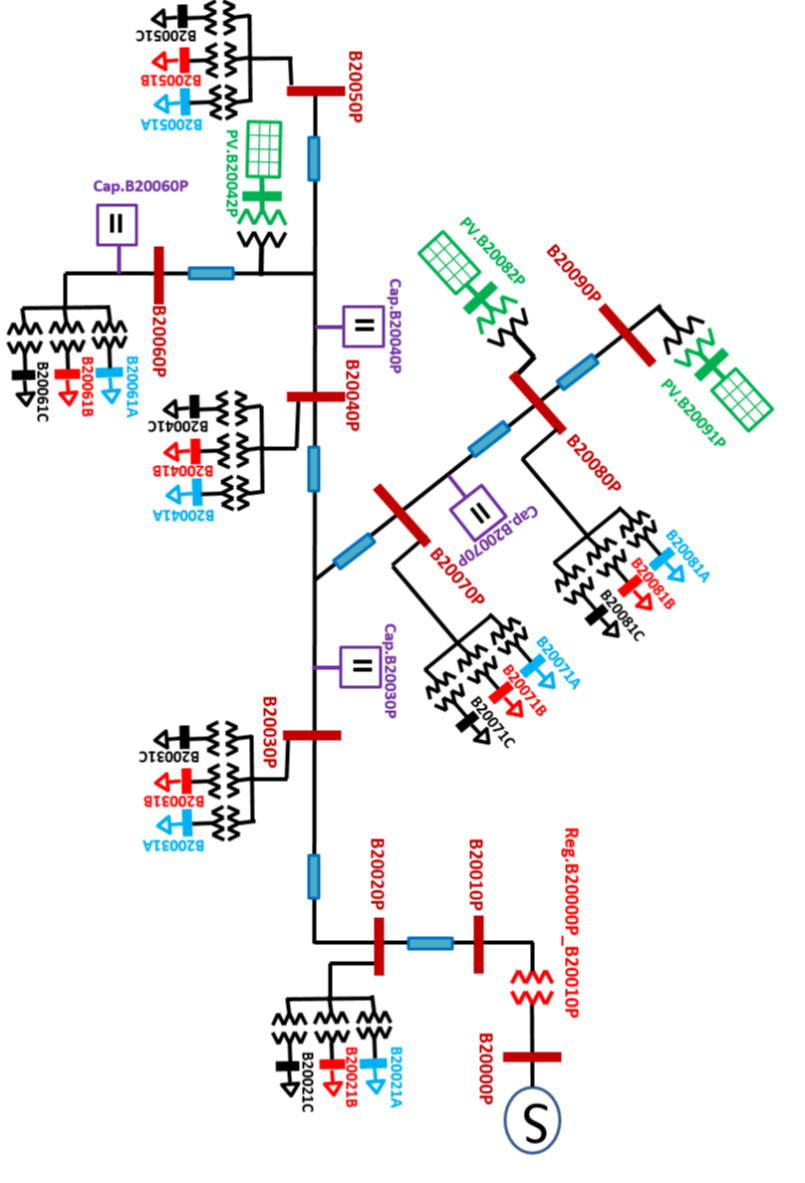
\includegraphics[width=0.9\linewidth]{figs/feeder_r.png} 
\caption{Distribution feeder used for validation}
\label{fig:feeder2}
\end{figure}

Fig. \ref{fig:without_vvc} shows the feeder voltage without coordinated voltage control during normal operation for one day. The dashed line on top represents the Upper limit (UL) for the voltage and the dashed line at the bottom represents the lower limit (LL) for the voltage. The upper and lower limits are set as 1.05 PU and 0.95 PU respectively. The solid lines represent voltages of busses B20010P to B20090P. They are labeled as V1 for bus B20010P, V2 bus for B20020P, V3 for bus B20030P and so on. As it can be seen in Fig. \ref{fig:without_vvc} the voltage profiles go above 1.06 PU and as low as 0.92 PU during regular operations during the 24-hour run. 
Fig. \ref{fig:with_cvc} shows the feeder voltages with coordinated voltage control implemented. It can be seen that the coordinated voltage control scheme is able to maintain the voltages within the UL and LL. This is possible by coordinating the use of the reactive power generation capabilities of the DG inverters with the traditional regulation devices. The reactive power supplied by the DG inverters are shown in Fig. \ref{fig:DG_Q}. Here QPV1, QPV2, and QPV3 represent the reactive power supplied by the inverter interfaced PVs located at bus B20040P, B20080P, and B20090P respectively. It can be observed that the DG interfaced inverters provide proper positive and negative reactive power compensation to compensate for voltage violation. The capacitor bank operations are shown in Fig. \ref{fig:cap_bank}. Here CAP1, CAP2, and CAP3 represent the capacitor banks located at bus B20040P, B20030P and B20070P respectively. The capacitor bank located at bus B20060P is defined as always on in the circuit configuration. So it is not considered in the control scheme. It can be observed in Fig. \ref{fig:cap_bank} that the capacitor banks closest to the nodes with voltage violation (CAP1 and CAP3) are being turned off during upper limit violation and during the lower limit violation CAP3 in being turned back on to deal with the lower limit violation. It should be noted there was no need for an OLTC operation to mitigate the voltage violation. This shows that with proper coordination of available resources the operation of mechanical regulation devices can be minimized increasing their life span and reducing the cost of operation. In the offline simulation, the CVC algorithm was fed the real, reactive power data as well as the voltage and current magnitude and angle data from all the nodes directly from the simulation. So the power-flow step shown in Fig. \ref{fig:Overview} was skipped in the off-line implementation as all the required data were considered to be available directly from the system. Also, the algorithm was executed for every simulation step synchronously with the power system simulation. This simulation was performed as an initial validation of the CVC algorithm for rapid prototyping. To see the behavior of the CVC algorithm in a more practical scenario real-time validation was performed.

\begin{figure}[!htb]
\centering
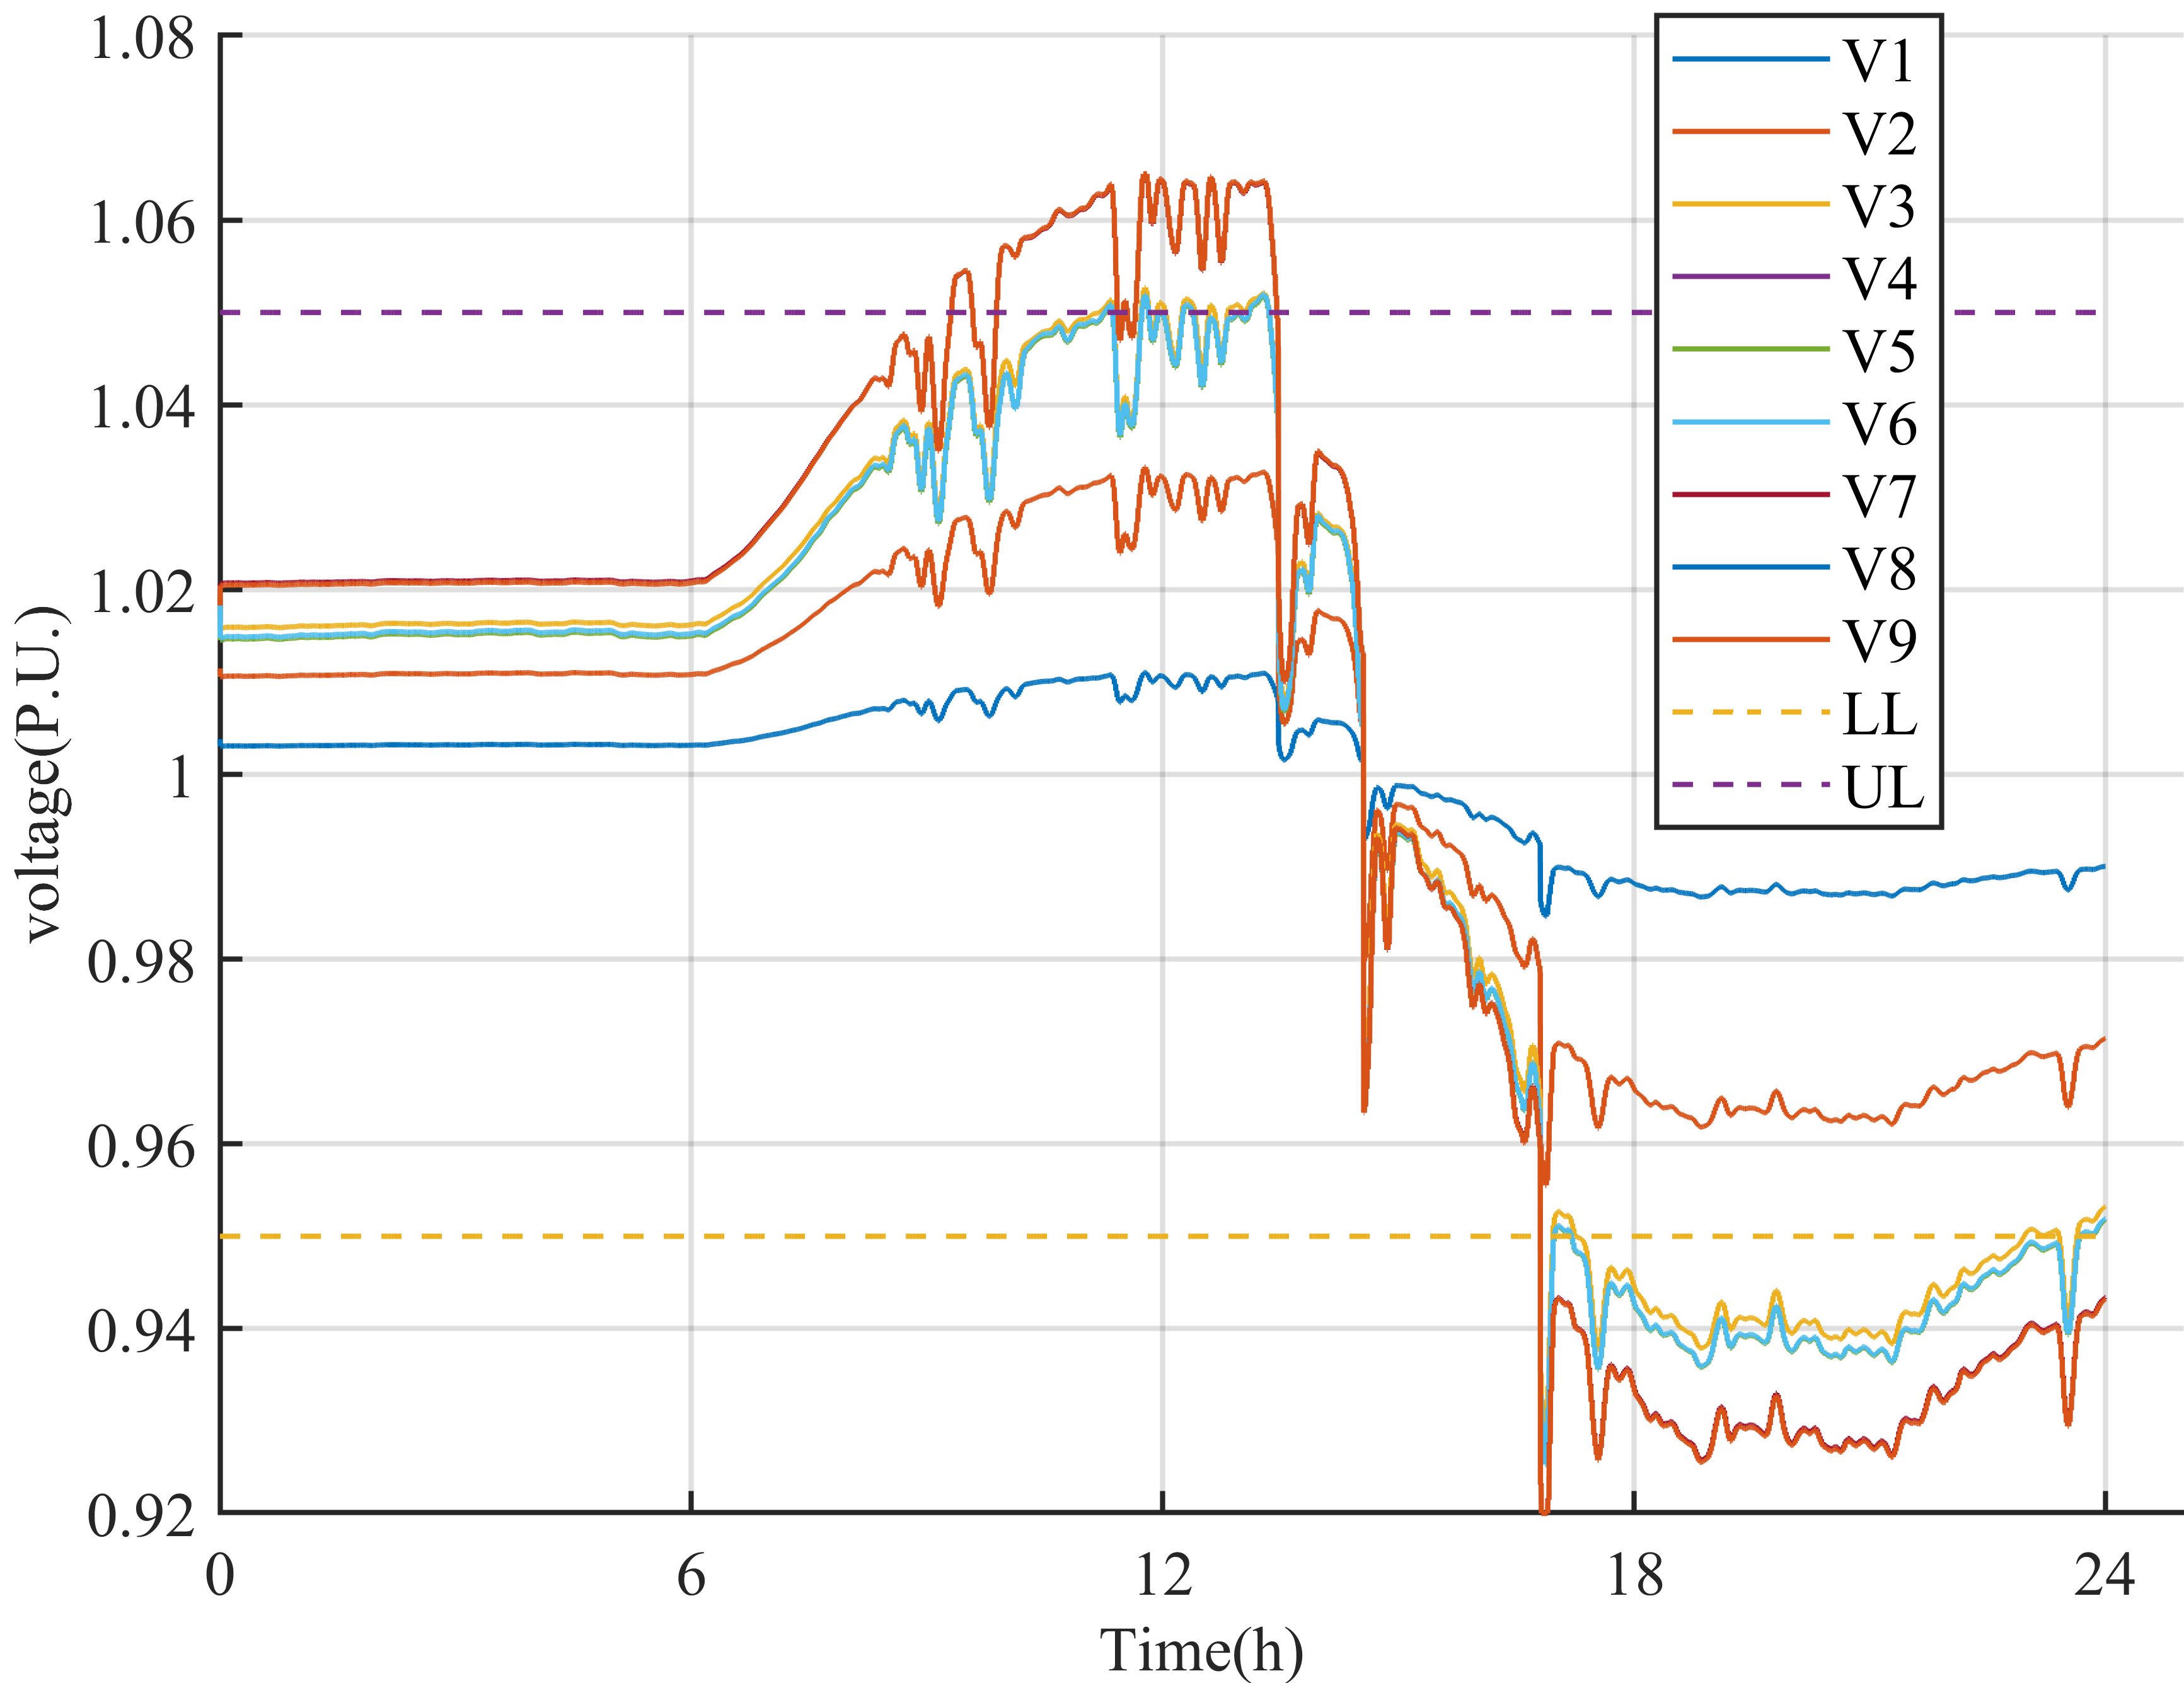
\includegraphics[width=\linewidth]{figs/NEW_WITHOUT_VVC.png}
\caption{Voltage Profile without Coordinated Voltage Control}
\label{fig:without_vvc}
\end{figure}

\begin{figure}[!htb]
\centering
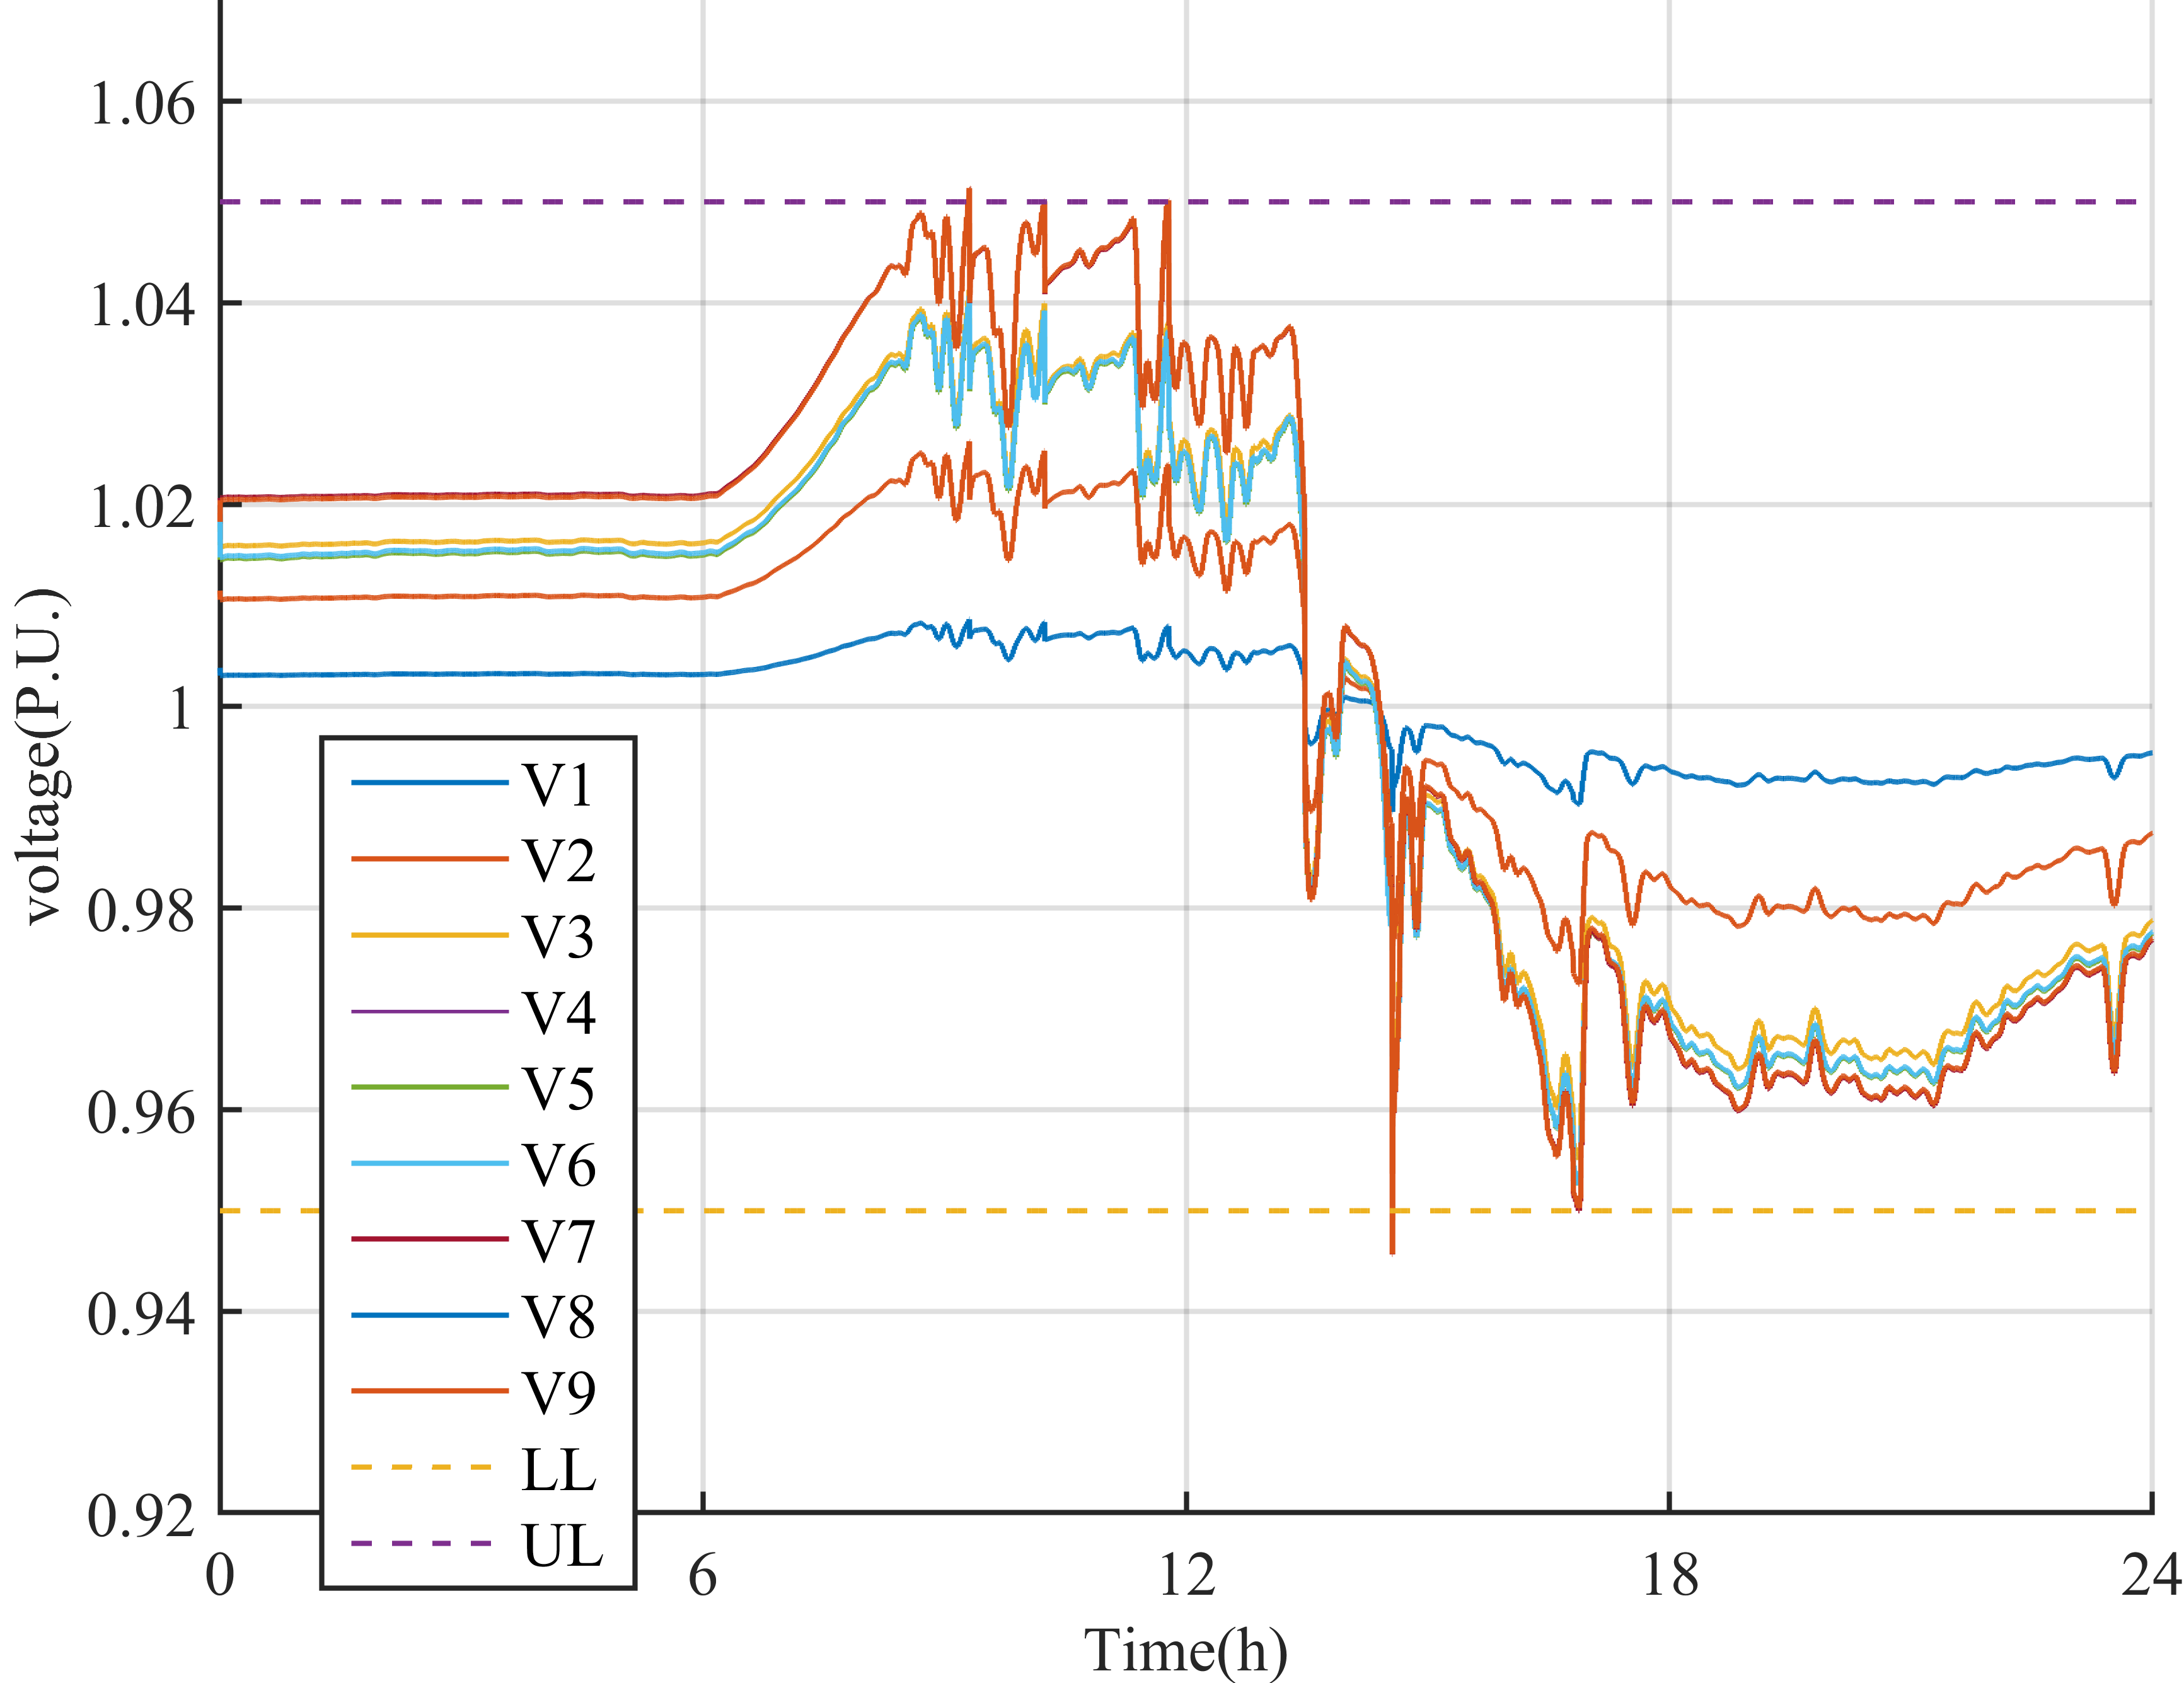
\includegraphics[width=\linewidth]{figs/NEW_WITH_VVC.png}
\caption{Voltage profile with coordinated voltage control}
\label{fig:with_cvc}
\end{figure}


\begin{figure}[!htb]
\centering
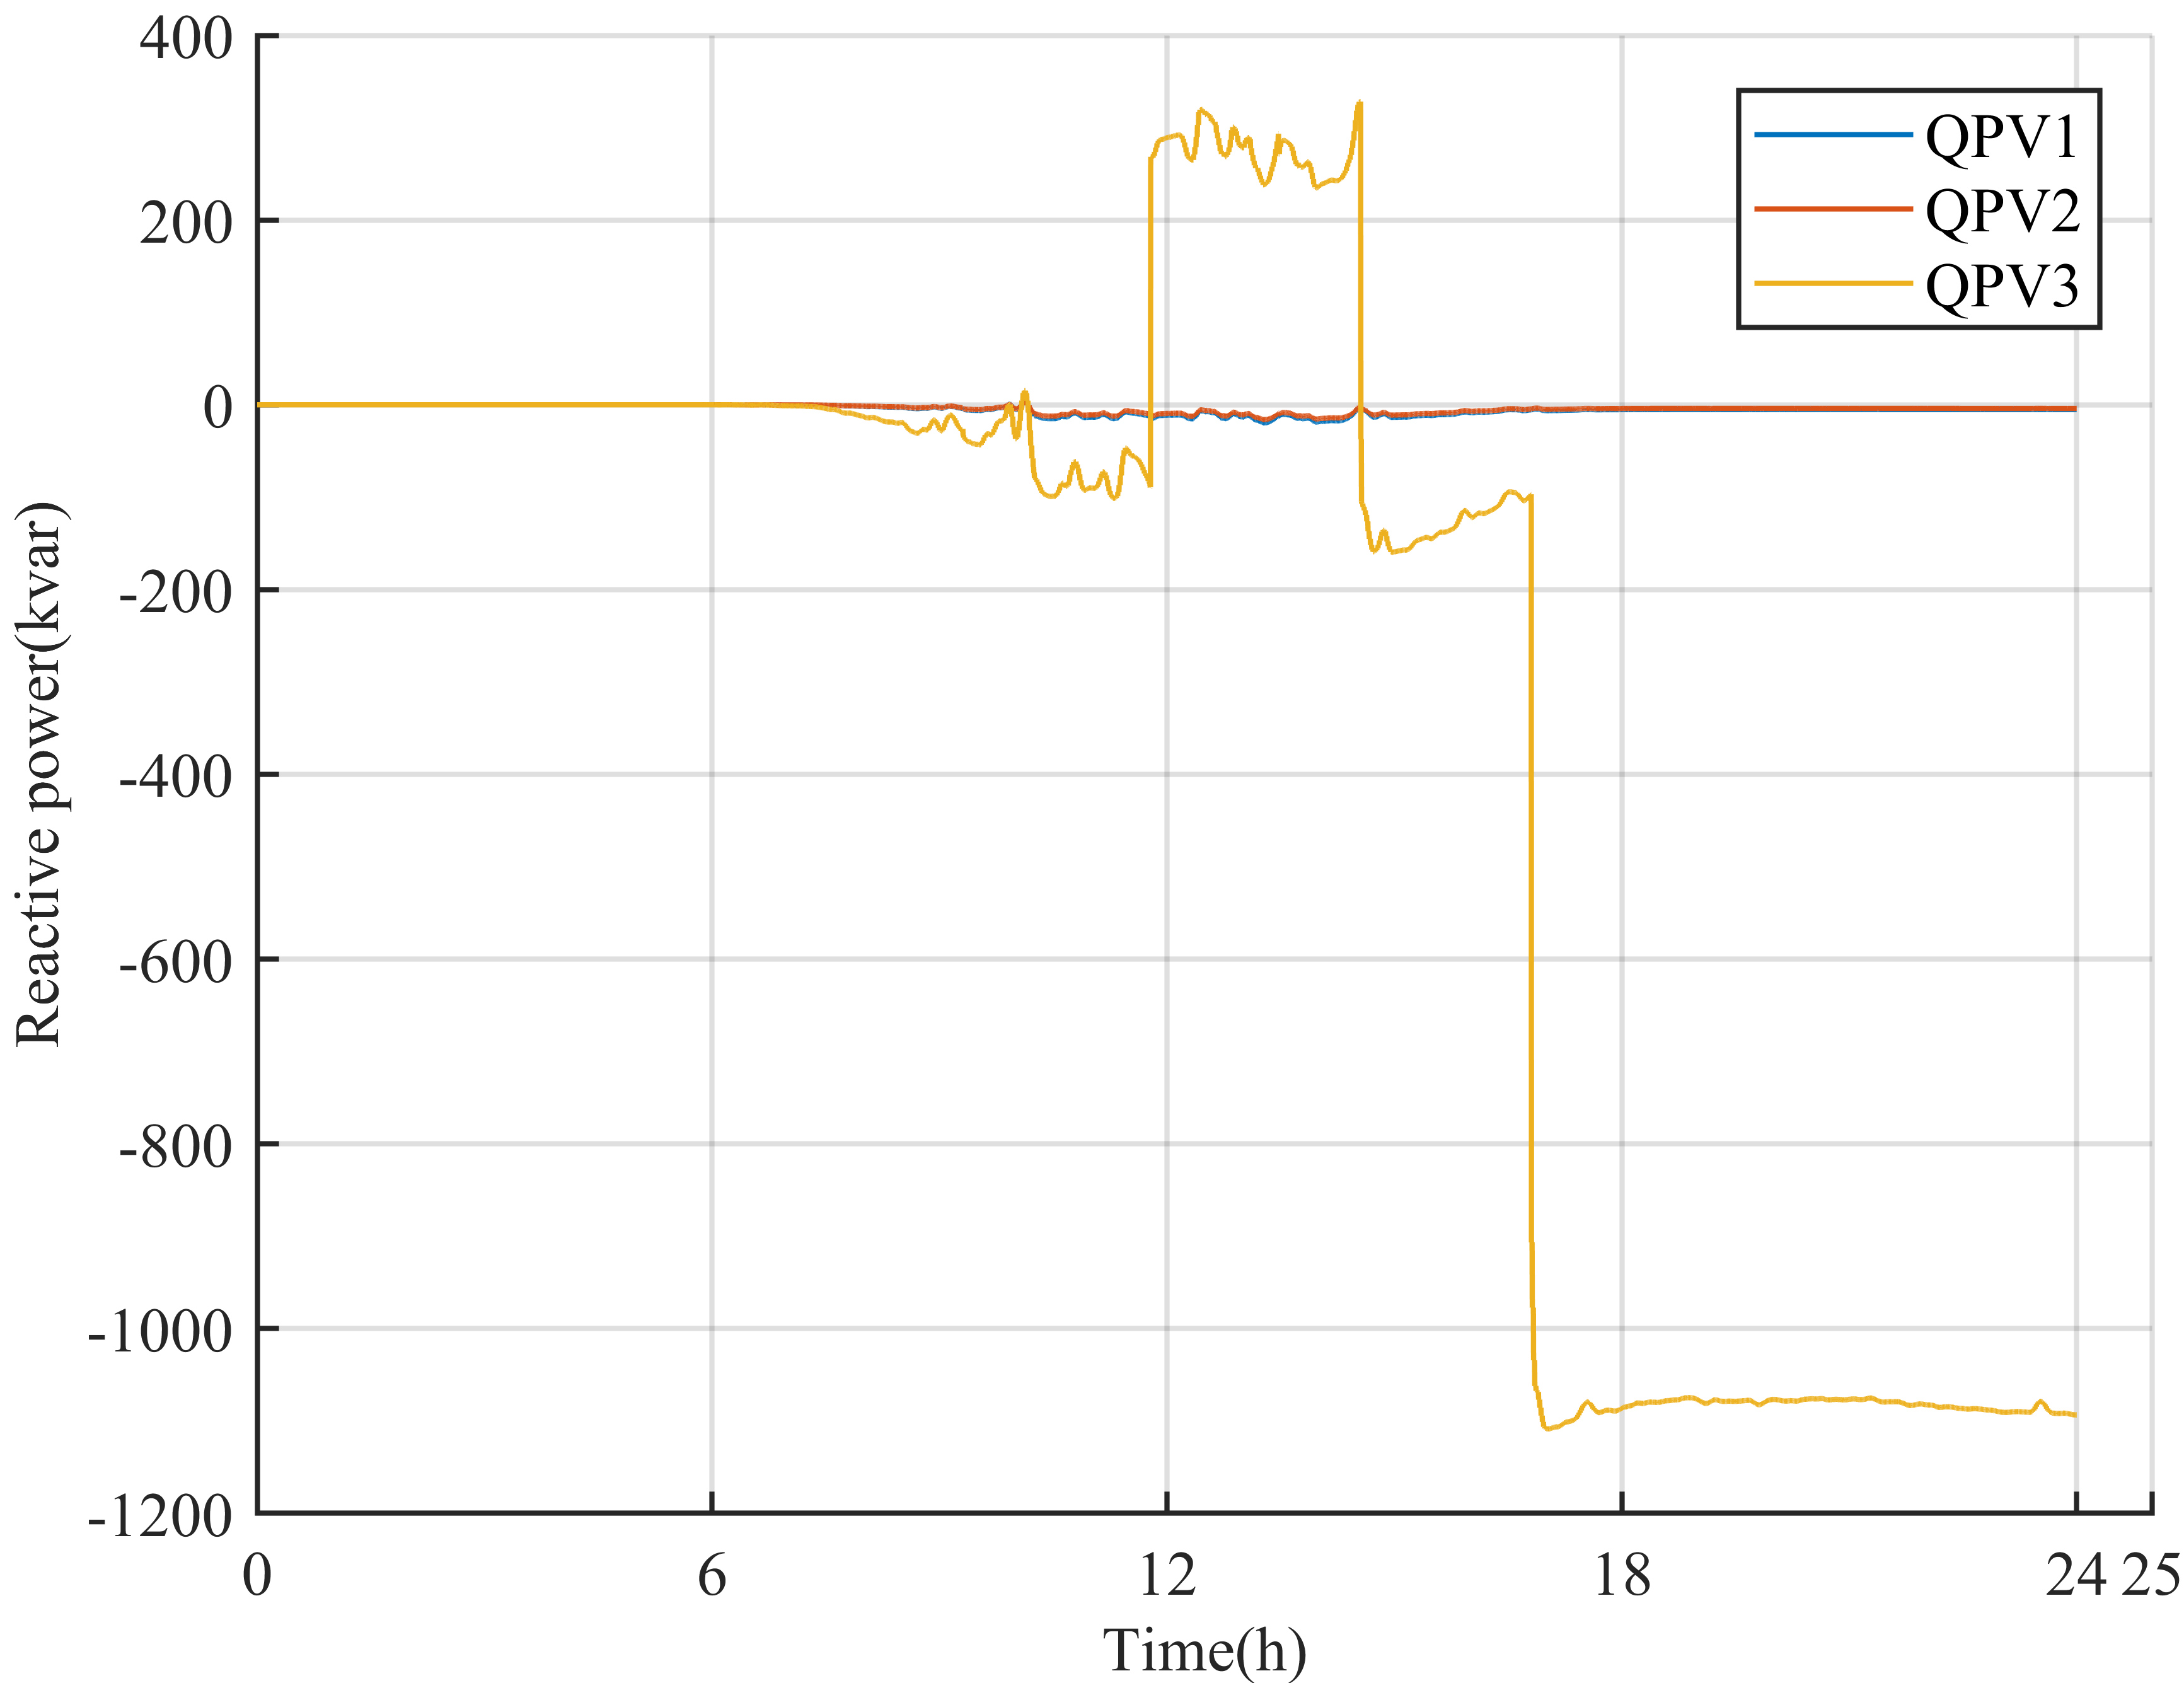
\includegraphics[width=\linewidth]{figs/NEW_PQ.png}
\caption{Reactive power supplied by DGs}
\label{fig:DG_Q}
\end{figure}

\begin{figure}[!htb]
\centering
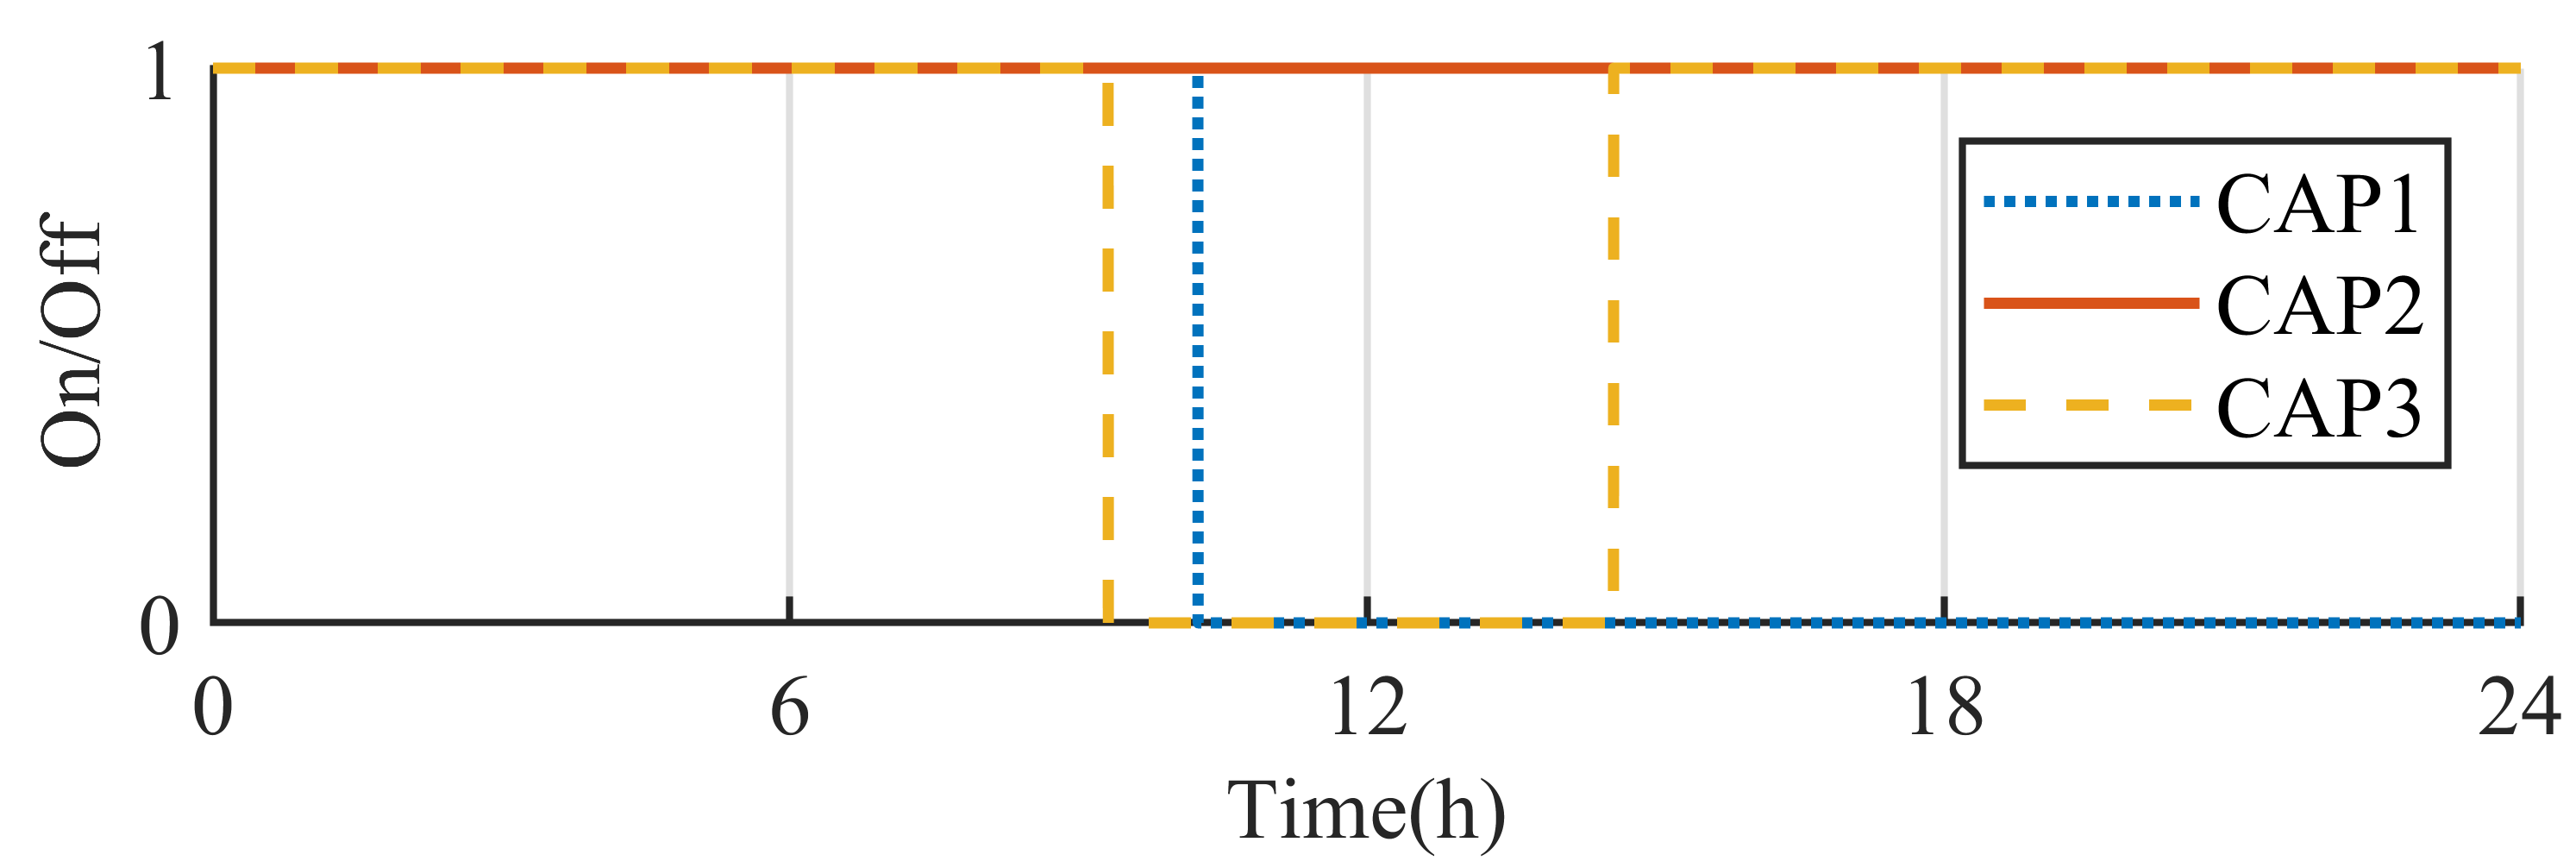
\includegraphics[width=\linewidth]{figs/NEW_CAPS.png}
\caption{Capacitor bank switching states}
\label{fig:cap_bank}
\end{figure}